\documentclass{article}

\usepackage{graphicx}
\usepackage{tikz}
\usepackage{tikzsymbols}
\usetikzlibrary{calc,patterns,shapes.geometric}
\pagestyle{empty}
\usepackage[margin=0pt]{geometry}
\geometry{papersize={14in,12in}}

\def\centerarc[#1](#2)(#3:#4:#5){\draw[#1] ($(#2)+({#5*cos(#3)},{#5*sin(#3)})$) arc (#3:#4:#5);}

\begin{document}
	\begin{figure}
		\centering
		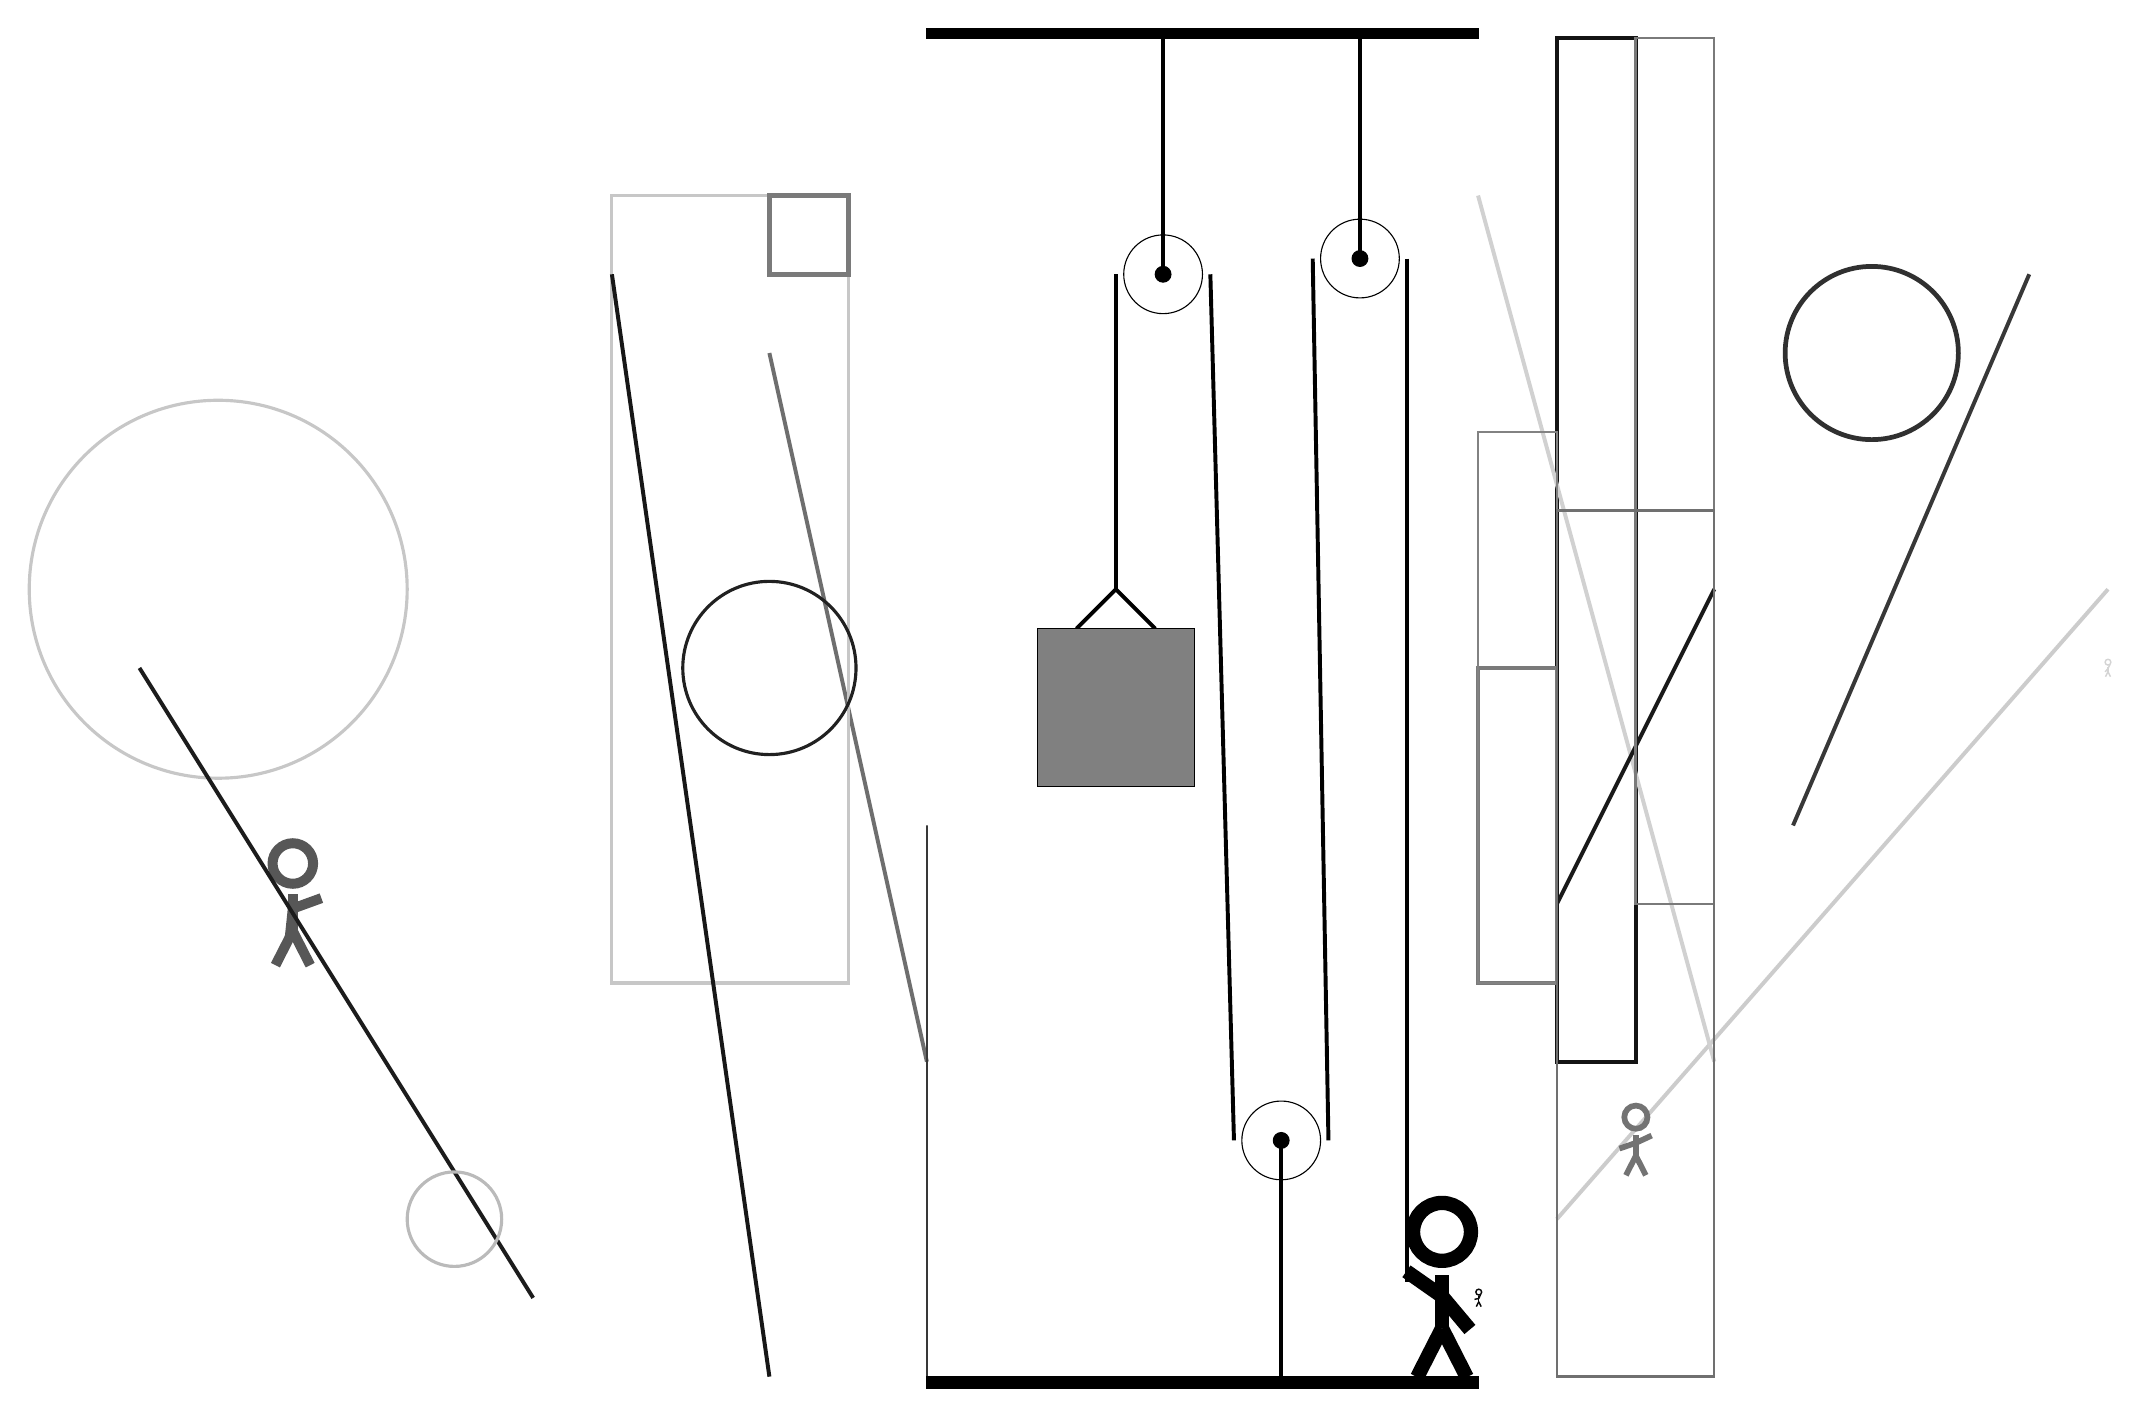
\begin{tikzpicture}
			%%%%% START %%%%%
			
			\draw[fill=black] (-2, 14) rectangle (5, 14.125);
			
			\draw (1, 11) circle (0.5);
			\draw[fill=black] (1, 11) circle (0.1);
			\draw[line width=0.5mm]  (1, 14) -- (1, 11);
			
			\draw[fill=white](2.5, 0) circle (0.5);
			\draw[fill=black] (2.5, 0) circle (0.1);
			\draw[line width=0.5mm]  (2.5, -3) -- (2.5, 0);
			
			\draw [line width=0.6mm, color=black!81](10, 10) circle (1.1);
			
			\draw[line width=0.5mm, color=black!92] (7, 14) rectangle (6, 1);
			\draw[line width=0.5mm, color=black!57](-2, 1) -- (-4, 10);
			\draw[line width=0.5mm, color=black!20](6, -1) -- (13, 7);
			\node[line width=0.5mm, color=black!66] at (-10, 3) {\Strichmaxerl[7][84][20]};
			\draw [line width=0.4mm, color=black!22](-11, 7) circle (2.4);
			\draw[line width=0.5mm, color=black!18](5, 12) -- (8, 1);
			\draw[line width=0.5mm, color=black!89](-7, -2) -- (-12, 6);
			\draw[line width=0.4mm, color=black!22] (-3, 12) rectangle (-6, 2);
			\draw[line width=0.5mm, color=black!90](6, 3) -- (8, 7);
			\draw [line width=0.4mm, color=black!27](-8, -1) circle (0.6);
			\node[line width=0.2mm, color=black!55] at (7, 0) {\Strichmaxerl[4][19][25]};
			\draw[line width=0.3mm, color=black!52] (7, 3) rectangle (8, 14);
			
			\node[line width=0.3mm, color=black!17] at (13, 6) {\Strichmaxerl[1][48][64]};
			\draw [line width=0.4mm, color=black!87](-4, 6) circle (1.1);
			\draw[line width=0.4mm, color=black!52] (5, 2) rectangle (6, 6);
			\draw[line width=0.6mm, color=black!52] (-3, 12) rectangle (-4, 11);
			
			\node[line width=0.3mm, color=black!97] at (5, -2) {\Strichmaxerl[1][11][65]};
			\draw[line width=0.5mm, color=black!78](9, 4) -- (12, 11);
			\draw[line width=0.5mm, color=black!91](-4, -3) -- (-6, 11);
			\draw[line width=0.3mm, color=black!49] (5, 2) rectangle (6, 9);
			
			\draw[line width=0.3mm, color=black!56] (6, 8) rectangle (8, -3);
			
			\draw[line width=0.3mm, color=black!78] (-2, 4) rectangle (-2, -3);
			
			\draw[fill=white](3.5, 11.2) circle (0.5);
			\draw[fill=black] (3.5, 11.2) circle (0.1);
			\draw[line width=0.5mm] (3.5, 14) -- (3.5, 11.2);
			
			\draw[line width=0.5mm] (-0.1, 6.5) -- (0.4, 7.0) -- (0.9, 6.5);
			\draw[fill=black!50] (-0.6, 6.5) rectangle (1.4, 4.5);
			
			\draw[line width=0.5mm] (0.4, 11) -- (0.4, 7.0);
			\centerarc[line width=0.5mm](1, 11)(0:180:0.6);
			\draw[line width=0.5mm](1.6, 11) -- (1.9, 0);
			\centerarc[line width=0.5mm](2.5, 0)(180:360:0.6);
			\draw[line width=0.5mm](3.1, 0) -- (2.9, 11.2);
			\centerarc[line width=0.5mm](3.5, 11.2)(0:180:0.6);
			\draw[line width=0.5mm](4.1, 11.2) -- (4.1, -1.8);
			
			\node at (4.5, -1.9) {\Strichmaxerl[10][-35][-50]};
			
			\draw[fill=black] (-2, -3) rectangle (5, -3.15);
			
			%%%%% END %%%%%
		\end{tikzpicture}
	\end{figure}	
\end{document}